\let\negmedspace\undefined
\let\negthickspace\undefined
\documentclass[journal]{IEEEtran}
\usepackage[a5paper, margin=10mm, onecolumn]{geometry}
%\usepackage{lmodern} % Ensure lmodern is loaded for pdflatex
\usepackage{tfrupee} % Include tfrupee package

\setlength{\headheight}{1cm} % Set the height of the header box
\setlength{\headsep}{0mm}     % Set the distance between the header box and the top of the text

\usepackage{gvv-book}
\usepackage{gvv}
\usepackage{cite}
\usepackage{amsmath,amssymb,amsfonts,amsthm}
\usepackage{algorithmic}
\usepackage{graphicx}
\usepackage{textcomp}
\usepackage{xcolor}
\usepackage{txfonts}
\usepackage{listings}
\usepackage{enumitem}
\usepackage{mathtools}
\usepackage{gensymb}
\usepackage{comment}
\usepackage[breaklinks=true]{hyperref}
\usepackage{tkz-euclide} 
\usepackage{listings}
% \usepackage{gvv}                                        
\def\inputGnumericTable{}                                 
\usepackage[latin1]{inputenc}                                
\usepackage{color}                                            
\usepackage{array}                                            
\usepackage{longtable}                                       
\usepackage{calc}                                             
\usepackage{multirow}                                         
\usepackage{hhline}                                           
\usepackage{ifthen}                                           
\usepackage{lscape}
\begin{document}

\bibliographystyle{IEEEtran}
\vspace{3cm}

\title{1.9.1}
\author{EE25BTECH11012-BEERAM MADHURI}
% \maketitle
% \newpage
% \bigskip
{\let\newpage\relax\maketitle}

\renewcommand{\thefigure}{\theenumi}
\renewcommand{\thetable}{\theenumi}
\setlength{\intextsep}{10pt} % Space between text and floats


\numberwithin{equation}{enumi}
\numberwithin{figure}{enumi}
\renewcommand{\thetable}{\theenumi}


\textbf{Question}:\\
The distance between the points $(m, -n)$ and $(-m, n)$ is \underline{\hspace{2cm}}.
\\
\textbf{Solution: }
let \textbf{A} and \textbf{B} be the vectors such that: 
\begin{table}[h!]
    \centering
    \begin{tabular}{|c|c|c|c|}
\hline
Angle (\(\alpha\)) & \(\cos(\alpha)\) & Value & Axis \\
\hline
\(90^\circ\) & \(\cos(90^\circ) = 0\) & \(l = 0\) & x-axis \\
\(60^\circ\) & \(\cos(60^\circ) = \frac{1}{2}\) & \(m = \frac{1}{2}\) & y-axis \\
\(30^\circ\) & \(\cos(30^\circ) = \frac{\sqrt{3}}{2}\) & \(n = \frac{\sqrt{3}}{2}\) & z-axis \\
\hline
\end{tabular}
    \caption{Variables used}
    \label{table 1.9.1}
\end{table}

Distance between \textbf{A} and \textbf{B} or Norm of \textbf{A} - \textbf{B} is:
\begin{align*}
\| \textbf{A} - \textbf{B} \| &= \sqrt{\|\textbf{A}\|^2 + \|\textbf{B}\|^2 - 2 A^\top\textbf{B} }\\
&= \sqrt{(m^2 + n^2) - 2(-m^2 - n^2) + m^2 + n^2} \\
&= \sqrt{4(m^2+n^2)} \\
&= 2\sqrt{m^2+n^2}
\end{align*}

Hence Distance between \textbf{A} and \textbf{B} is $2\sqrt{m^2+n^2}$.
\begin{figure}[h!]
    \centering
    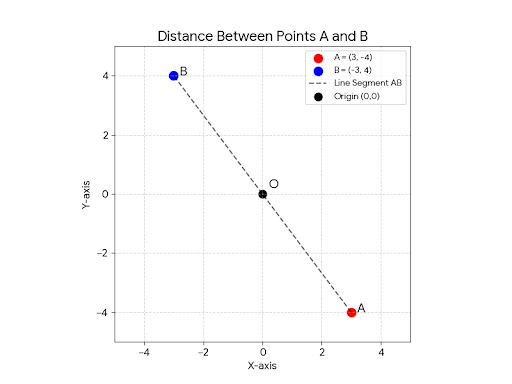
\includegraphics[width=0.7\columnwidth]{figs/graph.png}
    \caption{Plot}
    \label{fig:placeholder}
\end{figure}

\end{document}